%%%%%%%%%%%%%%%%%%%%%%%%%%%%%%%%%%%%%%%%%
% Beamer Presentation
% LaTeX Template
% Version 2.0 (March 8, 2022)
%
% This template originates from:
% https://www.LaTeXTemplates.com
%
% Author:
% Vel (vel@latextemplates.com)
%
% License:
% CC BY-NC-SA 4.0 (https://creativecommons.org/licenses/by-nc-sa/4.0/)
%
%%%%%%%%%%%%%%%%%%%%%%%%%%%%%%%%%%%%%%%%%

%----------------------------------------------------------------------------------------
%	PACKAGES AND OTHER DOCUMENT CONFIGURATIONS
%----------------------------------------------------------------------------------------

\documentclass[
	12pt, % Set the default font size, options include: 8pt, 9pt, 10pt, 11pt, 12pt, 14pt, 17pt, 20pt
	%t, % Uncomment to vertically align all slide content to the top of the slide, rather than the default centered
	%aspectratio=169, % Uncomment to set the aspect ratio to a 16:9 ratio which matches the aspect ratio of 1080p and 4K screens and projectors
]{beamer}

\graphicspath{{Images/}{./}} % Specifies where to look for included images (trailing slash required)

\usepackage{todonotes}
\usepackage{graphicx}
\usepackage{xcolor}
\usepackage{subfig}
%%\usepackage[noend]{algpseudocode}


\usepackage{algorithm}
\usepackage{algorithmic}

\usepackage{blkarray}
\usepackage{amsmath}
\usepackage{xspace}
\usepackage{float}


\usepackage{tikz}
\usetikzlibrary{matrix, decorations, patterns, positioning, shapes, calc, intersections, arrows, fit}

\usetikzlibrary{patterns}
\usetikzlibrary{fit,calc,positioning,decorations.pathreplacing,matrix}

\usepackage{booktabs} % Allows the use of \toprule, \midrule and \bottomrule for better rules in tables


\newcommand{\brown}[1]{{\color{brown} #1 }}


\definecolor{pastelgreen1}{rgb}{0.47, 0.87, 0.47}
\definecolor{pastelgreen}{rgb}{0, 1, 0}

\usetheme{Madrid}




%----------------------------------------------------------------------------------------
%	SELECT INNER THEME
%----------------------------------------------------------------------------------------

% Inner themes change the styling of internal slide elements, for example: bullet points, blocks, bibliography entries, title pages, theorems, etc. Uncomment each theme in turn to see what changes it makes to your presentation.

%\useinnertheme{default}
%\useinnertheme{circles}
%\useinnertheme{rectangles}
%\useinnertheme{rounded}
%\useinnertheme{inmargin}

%----------------------------------------------------------------------------------------
%	SELECT OUTER THEME
%----------------------------------------------------------------------------------------

% Outer themes change the overall layout of slides, such as: header and footer lines, sidebars and slide titles. Uncomment each theme in turn to see what changes it makes to your presentation.

%\useoutertheme{default}
%\useoutertheme{infolines}
%\useoutertheme{miniframes}
%\useoutertheme{smoothbars}
%\useoutertheme{sidebar}
%\useoutertheme{split}
%\useoutertheme{shadow}
%\useoutertheme{tree}
%\useoutertheme{smoothtree}


%----------------------------------------------------------------------------------------
%	PRESENTATION INFORMATION
%----------------------------------------------------------------------------------------

\title[Data-aware algorithms]{Data-aware algorithms for matrix and tensor computations} % The short title in the optional parameter appears at the bottom of every slide, the full title in the main parameter is only on the title page

%\subtitle{Optional Subtitle} % Presentation subtitle, remove this command if a subtitle isn't required

\author[Suraj Kumar]{Suraj Kumar} % Presenter name(s), the optional parameter can contain a shortened version to appear on the bottom of every slide, while the main parameter will appear on the title slide

\institute[Inria \& ENS Lyon]{Inria \& ENS Lyon \\ \smallskip Email:\textit{suraj.kumar@inria.fr}} % Your institution, the optional parameter can be used for the institution shorthand and will appear on the bottom of every slide after author names, while the required parameter is used on the title slide and can include your email address or additional information on separate lines

\date[CR12]{CR12: September 2023\\ \smallskip\small https://surakuma.github.io/courses/daamtc.html} % Presentation date or conference/meeting name, the optional parameter can contain a shortened version to appear on the bottom of every slide, while the required parameter value is output to the title slide

%----------------------------------------------------------------------------------------

\begin{document}

%----------------------------------------------------------------------------------------
%	TITLE SLIDE
%----------------------------------------------------------------------------------------

\begin{frame}
	\titlepage % Output the title slide, automatically created using the text entered in the PRESENTATION INFORMATION block above
\end{frame}

%----------------------------------------------------------------------------------------
%	TABLE OF CONTENTS SLIDE
%----------------------------------------------------------------------------------------

% The table of contents outputs the sections and subsections that appear in your presentation, specified with the standard \section and \subsection commands. You may either display all sections and subsections on one slide with \tableofcontents, or display each section at a time on subsequent slides with \tableofcontents[pausesections]. The latter is useful if you want to step through each section and mention what you will discuss.

\begin{frame}{Table of Contents} 
	\tableofcontents[currentsection] % Output the table of contents (all sections on one slide)
\end{frame}
\section{Course details}

\begin{frame}{Course details}

\brown{Topics:}
	\begin{itemize}
		\item Communication costs on sequential and parallel machines
		\item Matrix computations
		\item Tensor computations
		\item Popular ways to work with large matrix and tensor data
	\end{itemize}
\vfill
\brown{Class hours:} Tuesday 08:00 AM + Thursday  03:45 PM\\
\vfill
\brown{Location:} Room B1\\
\vfill
\brown{Contact:} suraj.kumar@inria.fr 
\end{frame}

\begin{frame}{Course details}

\brown{Evaluation:}
\begin{itemize}
	\item 3 homework assignments (40\%)
	\item Project (60\%): 1/2 students, paper(s) reading + report + presentation
\end{itemize}
\vfill
\brown{Website:}
\begin{itemize}
	\item \url{https://surakuma.github.io/courses/daamtc.html}
	\item Course material available online (right after class)
	\item Link to assignments and other resources
\end{itemize}
\vfill
\brown{General stuff:}
\begin{itemize}
	\item Stop me with questions, ask for re-explanation
	\item Will have catch-up sessions after each 2 weeks
	\item Feel free to email your doubts
\end{itemize}


\end{frame}



\section{Introduction \& Motivation}
\begin{frame}{Table of Contents} 
	\tableofcontents[currentsection] % Output the table of contents (all sections on one slide)
\end{frame}
\begin{frame}{Motivation}
	\begin{itemize}
		\item (Fast) Memory: place to store data to compute
		\vfill
		\item Always been a limited resource (4KB in Appollo 11 computer)
		\vfill
		\item 64KB L1 cache  in recent iphone 
		\vfill
		\item Problem size is always getting bigger ...
		\vfill
		\item Annual improvements:
		\begin{itemize}
			\item Time per flop (computation): 59\%
   			\item Data movement (communication):\\
			\begin{tabular}{c|c|c}
				& Bandwidth & Latency\\
				\hline
				Network & 26\% & 15\%\\
				DRAM & 23\% & 5\%\\
			\end{tabular}
		\end{itemize}
	\end{itemize}
	\footnotesize  Data from \textit{Getting up to speed: The future of supercomputing},
	2005, National Academies Press (2004 figure based on data on the
	period 1988-2002)
\end{frame}


\begin{frame}{Flop per byte moved ratio}
\centerline{\includegraphics[width=0.625\linewidth]{flop-per-byte-sp.png}}
{\tiny From \url{http://www.karlrupp.net/2013/06/cpu-gpu-and-mic-hardware-characteristics-over-time/}}
\begin{itemize}
	\item Number of flops performed in the time needed to move a byte
	\item $\frac{\textnormal{computing speed}}{\textnormal{communication speed}}$\\
	\item Avoid communication to save time (and energy)
\end{itemize}
\end{frame}
\begin{frame}{Simplified model for a sequential CPU core}
	\begin{minipage}[l]{0.56\linewidth}
		\vspace*{0.6cm}
		\begin{center}
			\begin{figure}
				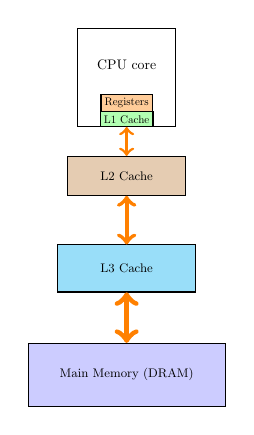
\begin{tikzpicture}[scale=0.5, every node/.style={transform shape}]
				%			\tikzstyle{taskmemory}=[draw=black, minimum height=10mm, minimum width=21mm, fill=blue!40, text=black]
				\tikzstyle{taskmemory}=[draw=black, minimum height=8mm, minimum width=25mm, fill=blue!20, text=black]
				\tikzstyle{taskcompute}=[draw=black, minimum height=25mm, minimum width=25mm, fill=none, text=black, below]
				
				\node (t0) at (0,0) [taskcompute] {}; 
%				\node (t1) at (0,-4) [taskmemory] {$DRAM$};
%				
%				
%				\draw [<->, line width=1, orange] (t0) -- (t1);

   				 \node[above, draw, rectangle, scale=0.8, fill=green!30] (lc1) at (t0.south) {$\textnormal{L1 Cache}$};
   				 \node[above, draw, rectangle, scale=0.8, fill=orange!40] (lregister) at (lc1.north) {$\textnormal{Registers}$};
		    	\node [above] at (t0.mid) {$\textnormal{CPU core}$};
		    	
		    	
 				\node (L2cache) at (0,-3.25) [taskcompute, minimum width=30mm, minimum height=10mm, fill=brown!40] {\small$\textnormal{L2 Cache}$}; 

				\draw [<->, line width=1, orange] (t0) -- (L2cache);
				
 				\node (L3cache) at (0,-5.5) [taskcompute, minimum width=35mm, minimum height=12mm, fill=cyan!40] {\small$\textnormal{L3 Cache}$}; 
				\draw [<->, line width=1.5, orange] (L2cache) -- (L3cache);
				
				\node (mainmemory) at (0,-8) [taskcompute, minimum width=50mm, minimum height=16mm, fill=blue!20] {\small$\textnormal{Main Memory (DRAM)}$}; 
				\draw [<->, line width=2, orange] (L3cache) -- (mainmemory);		    	
		    	
		    	
%				
%				
%				\node (td0)  at (t0.south) [above, scale=0.6] {$Cache$};
%%				%			\node (td1) [above, scale=0.6] at (t1.south) {$DRAM$};
%%				%			\node (td2) [above, scale=0.6] at (t2.south) {$DRAM$};
%%				%			\node (td3) [above, scale=0.6] at (t3.south) {$DRAM$};
%				
%				\node [above] at (td0.north) {$\textnormal{CPU core}$};
%				
				
				%		\path (0, -2) -- (0.1, -2);
				%		\path (0, 6) -- (0.1, 6);
				
				\end{tikzpicture}
				
				\centering{\scriptsize Cache hierarchy model}
			\end{figure}
		\end{center}
	\end{minipage}
\hfill
\begin{minipage}{0.4\linewidth}
	
	\vfill
			\begin{center}
		\begin{figure}
			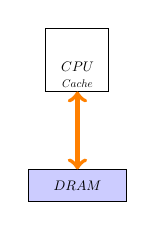
\begin{tikzpicture}[scale=0.5, every node/.style={transform shape}]
			%			\tikzstyle{taskmemory}=[draw=black, minimum height=10mm, minimum width=21mm, fill=blue!40, text=black]
			\tikzstyle{taskmemory}=[draw=black, minimum height=8mm, minimum width=25mm, fill=blue!20, text=black]
			\tikzstyle{taskcompute}=[draw=black, minimum height=16mm, minimum width=16mm, fill=none, text=black, below]
			
			\node (t0) at (0,4) [taskcompute] {}; 
			\node (t1) at (0,0) [taskmemory] {$DRAM$};
			
			
			\draw [<->, line width=1.5, orange] (t0) -- (t1);
			
			
			\node (td0)  at (t0.south) [above, scale=0.8] {$Cache$};
			%			\node (td1) [above, scale=0.6] at (t1.south) {$DRAM$};
			%			\node (td2) [above, scale=0.6] at (t2.south) {$DRAM$};
			%			\node (td3) [above, scale=0.6] at (t3.south) {$DRAM$};
			
			\node [above] at (td0.north) {$CPU$};
			
			
			%		\path (0, -2) -- (0.1, -2);
			%		\path (0, 6) -- (0.1, 6);
			
			\end{tikzpicture}
			
			\centering{\scriptsize Simplified model}
		\end{figure}
	\end{center}
\end{minipage}

%\vfill
%\begin{itemize}
%	\item A simplified data transfer model for a CPU core
%\end{itemize}
\end{frame}


\begin{frame}{Shared memory machine model}
		\begin{center}
	\begin{figure}
		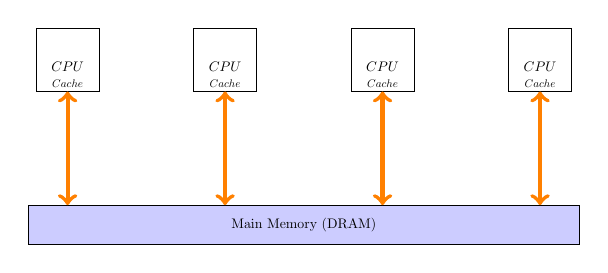
\begin{tikzpicture}[scale=0.5, every node/.style={transform shape}]
		%			\tikzstyle{taskmemory}=[draw=black, minimum height=10mm, minimum width=21mm, fill=blue!40, text=black]
		\tikzstyle{taskmemory}=[draw=black, minimum height=10mm, minimum width=25mm, fill=blue!20, text=black]
		\tikzstyle{taskcompute}=[draw=black, minimum height=16mm, minimum width=16mm, fill=none, text=black, below]
		
		\node (t0) at (0,0) [taskcompute] {}; 
		\node (t1) at (4,0) [taskcompute] {};
		\node (t2) at (8,0) [taskcompute] {};
		\node (t3) at (12,0) [taskcompute] {};   

		
		
		\node (td0)  at (t0.south) [above, scale=0.8] {$Cache$};
		\node [above] at (td0.north) {$CPU$};
		
		\node (td1)  at (t1.south) [above, scale=0.8] {$Cache$};
		\node [above] at (td1.north) {$CPU$};
		
		\node (td2)  at (t2.south) [above, scale=0.8] {$Cache$};
		\node [above] at (td2.north) {$CPU$};
		
		\node (td3)  at (t3.south) [above, scale=0.8] {$Cache$};
		\node [above] at (td3.north) {$CPU$};
		
		\node (tmemory) at (6,-5) [taskmemory, minimum width=140mm] {$\textnormal{Main Memory (DRAM)}$};
		\draw [<->, line width=1.5, orange] (t0) -- (0,-4.5);
		\draw [<->, line width=1.5, orange] (t1) -- (4,-4.5);
		\draw [<->, line width=1.5, orange] (t2) -- (8,-4.5);
		\draw [<->, line width=1.5, orange] (t3) -- (12,-4.5);
								
		\end{tikzpicture}
		
		\centering{\scriptsize Shared memory parallel machine model}
	\end{figure}
\end{center}

\begin{itemize}
	\item We can view all CPUs as a single large processing unit
\end{itemize}
\end{frame}

\begin{frame}{Data transfer models in this course}

\begin{minipage}[l]{0.4\linewidth}
	\begin{center}
		\begin{figure}
			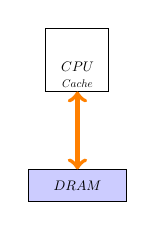
\begin{tikzpicture}[scale=0.5, every node/.style={transform shape}]
			%			\tikzstyle{taskmemory}=[draw=black, minimum height=10mm, minimum width=21mm, fill=blue!40, text=black]
			\tikzstyle{taskmemory}=[draw=black, minimum height=8mm, minimum width=25mm, fill=blue!20, text=black]
			\tikzstyle{taskcompute}=[draw=black, minimum height=16mm, minimum width=16mm, fill=none, text=black, below]
			
			\node (t0) at (0,4) [taskcompute] {}; 
			\node (t1) at (0,0) [taskmemory] {$DRAM$};
			
			
			\draw [<->, line width=1.5, orange] (t0) -- (t1);
			
			
			\node (td0)  at (t0.south) [above, scale=0.8] {$Cache$};
			\node [above] at (td0.north) {$CPU$};
			
			\end{tikzpicture}
			
			\centering{\scriptsize Sequential machine}
		\end{figure}
	\end{center}
\end{minipage}
\hfill
\begin{minipage}{0.45\linewidth}
	\begin{center}
		\begin{figure}
			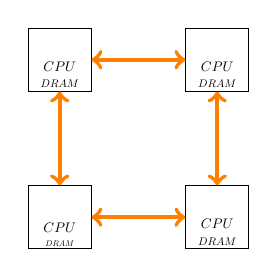
\begin{tikzpicture}[scale=0.5, every node/.style={transform shape}]
			%%\tikzstyle{taskmemory}=[draw=black, minimum height=18mm, minimum width=18mm, fill=blue!40, text=black]
			\tikzstyle{taskcompute}=[draw=black, minimum height=16mm, minimum width=16mm, fill=none, text=black, below]
			
			\node (t0) at (0,0) [taskcompute] {}; 
			\node (t1) at (4,0) [taskcompute] {};
			\node (t2) at (4,4) [taskcompute] {};
			\node (t3) at (0,4) [taskcompute] {};
			
			\draw [<->, line width=1.5, orange] (t0) -- (t1);
			\draw [<->, line width=1.5, orange] (t1) -- (t2);
			\draw [<->, line width=1.5, orange] (t2) -- (t3);
			\draw [<->, line width=1.5, orange] (t3) -- (t0);
			
			%%\draw [<->, line width=3, orange] (t0) -- (t2);
			%%\draw [<->, line width=3, orange] (t1) -- (t3);
			
			\node (td0)  at (t0.south) [above, scale=0.6] {$DRAM$};
			\node (td1) [above, scale=0.8] at (t1.south) {$DRAM$};
			\node (td2) [above, scale=0.8] at (t2.south) {$DRAM$};
			\node (td3) [above, scale=0.8] at (t3.south) {$DRAM$};
			
			\node [above] at (td0.north) {$CPU$};
			\node [above] at (td1.north) {$CPU$};
			\node [above] at (td2.north) {$CPU$};
			\node [above] at (td3.north) {$CPU$};
			
			%		\path (0, -2) -- (0.1, -2);
			%		\path (0, 6) -- (0.1, 6);
			\end{tikzpicture}
			
			\centering{\scriptsize Distributed memory homogeneous machine}
		\end{figure}
	\end{center}
\end{minipage}
\vfill
\begin{itemize}
	\item $\alpha$: per-message latency cost, $\beta$: per-word bandwidth cost, $\gamma$: per-operation arithmetic cost
	\item An algorithm's total cost = $\alpha \cdot$ (\#messages) + $\beta\cdot$(\#data transfers) + $\gamma \cdot$ (\#computations)
	\item For a parallel machine, we consider cost along the critical path
%	\item  
\end{itemize}
\vfill
{\footnotesize Sometimes computations can be overlapped with data transfers. However to keep the models simple we will not take that into account through out the course.} 

\end{frame}



\begin{frame}{Tensors and their uses}
		\begin{center}
	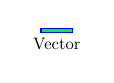
\begin{tikzpicture}[scale=0.1, every node/.style={transform shape}]
	\pgfmathsetmacro{\rectx}{4}
	\pgfmathsetmacro{\recty}{0.5}
	\draw[blue,fill=pastelgreen] (0,0) -- node [below, scale=6, black] {Vector}++(-\rectx,0) -- ++(0,\recty) -- ++(\rectx, 0) -- cycle;
	\end{tikzpicture}$\;$
	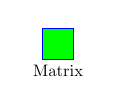
\begin{tikzpicture}[scale=0.1, every node/.style={transform shape}]
	\pgfmathsetmacro{\rectx}{4}
	\pgfmathsetmacro{\recty}{4}
	\draw[blue,fill=pastelgreen] (0,0) -- node [below, scale=6, black] {Matrix}++(-\rectx,0) -- ++(0,\recty) -- ++(\rectx, 0) -- cycle;
	%%\addvmargin{4};
	\end{tikzpicture}$\;$
	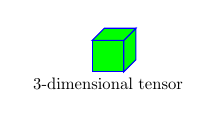
\begin{tikzpicture}[scale=0.1, every node/.style={transform shape}]
	\pgfmathsetmacro{\cubex}{4}
	\pgfmathsetmacro{\cubey}{4}
	\pgfmathsetmacro{\cubez}{4}
	\draw[blue,fill=pastelgreen] (0,0,0) -- ++(-\cubex,0,0) -- ++(0,-\cubey,0) --node [below, scale=6, black] {3-dimensional tensor} ++(\cubex,0,0) -- cycle;
	\draw[blue,fill=pastelgreen] (0,0,0) -- ++(0,0,-\cubez) -- ++(0,-\cubey,0) -- ++(0,0,\cubez) -- cycle;
	\draw[blue,fill=pastelgreen] (0,0,0) -- ++(-\cubex,0,0) -- ++(0,0,-\cubez) -- ++(\cubex,0,0) -- cycle;
	\end{tikzpicture}$\;$
	%%	\end{center}
	%%	\begin{center}	
	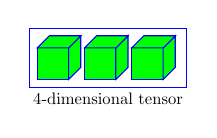
\begin{tikzpicture}[scale=0.1, every node/.style={transform shape}]
	\pgfmathsetmacro{\cubex}{4}
	\pgfmathsetmacro{\cubey}{4}
	\pgfmathsetmacro{\cubez}{4}
	\draw[blue,fill=pastelgreen] (0,0,0) -- ++(-\cubex,0,0) -- ++(0,-\cubey,0) -- ++(\cubex,0,0) -- cycle;
	\draw[blue,fill=pastelgreen] (0,0,0) -- ++(0,0,-\cubez) -- ++(0,-\cubey,0) -- ++(0,0,\cubez) -- cycle;
	\draw[blue,fill=pastelgreen] (0,0,0) -- ++(-\cubex,0,0) -- ++(0,0,-\cubez) -- ++(\cubex,0,0) -- cycle;
	
	\draw[blue,fill=pastelgreen] (\cubex +2,0,0) -- ++(-\cubex,0,0) -- ++(0,-\cubey,0) -- ++(\cubex,0,0) -- cycle;
	\draw[blue,fill=pastelgreen] (\cubex +2,0,0) -- ++(0,0,-\cubez) -- ++(0,-\cubey,0) -- ++(0,0,\cubez) -- cycle;
	\draw[blue,fill=pastelgreen] (\cubex +2,0,0) -- ++(-\cubex,0,0) -- ++(0,0,-\cubez) -- ++(\cubex,0,0) -- cycle;
	
	\draw[blue,fill=pastelgreen] (\cubex +2 + \cubex +2,0,0) -- ++(-\cubex,0,0) -- ++(0,-\cubey,0) -- ++(\cubex,0,0) -- cycle;
	\draw[blue,fill=pastelgreen] (\cubex +2 + \cubex +2,0,0) -- ++(0,0,-\cubez) -- ++(0,-\cubey,0) -- ++(0,0,\cubez) -- cycle;
	\draw[blue,fill=pastelgreen] (\cubex +2 + \cubex +2,0,0) -- ++(-\cubex,0,0) -- ++(0,0,-\cubez) -- ++(\cubex,0,0) -- cycle;
	
	\draw[blue, fill=none] (-\cubex -1, 2.5, 0) -- ++(0, -\cubey -3.5, 0) --node [below, scale=6, black] {4-dimensional tensor} ++(\cubex +2 + \cubex +2 + \cubex + \cubex,0,0) -- ++(0, \cubey +3.5, 0) -- cycle; 
	
	%%\node [scale=2] at (0, -8) {$hello$};
	\end{tikzpicture}
\end{center}



		\begin{itemize}
			\item \textbf{Neuroscience}: Neuron $\times$ Time $\times$ Trial
			%%		\item \textbf{Transportation}: Pickup $\times$ Dropoff $\times$ Time
			\item \textbf{Media}: User x Movie x Time 
			\item \textbf{Ecommerce}: User x Product x Time
			\item \textbf{Social-Network}: Person x Person x Time x Type
			%%		\item[$\textcolor{blue}{\bullet}$] \textbf{Social-Network}: Person x Person x Time x Type
		\end{itemize}
%	\end{minipage}
%	\begin{minipage}{1.0\linewidth}


	

\end{frame}

\begin{frame}{Tensors and their uses}
	\begin{itemize}
	\vfill
	\item High dimensional tensors: Neural network, Molecular simulation, Quantum computing
	\vfill
	\item People work with low dimensional structure (decomposition) of the tensors
	\begin{center}
		\begin{columns}
			\hfill\begin{column}{0.365\linewidth}
				\begin{block}{\scriptsize Canonical decomposition}
					\begin{center}
						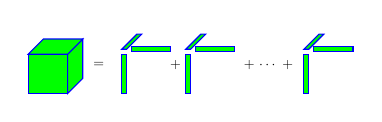
\begin{tikzpicture}[scale=0.125, every node/.style={transform shape}]
						%%						\pgfmathsetmacro{\cubex}{2}
						%%						\pgfmathsetmacro{\cubey}{2}
						%%						\pgfmathsetmacro{\cubez}{2}
						%%						\path (0,0,-\cubez-1) -- ++(-\cubex,0,0) -- ++(0,0,-\cubez-2) -- ++(\cubex,0,0) -- cycle;
						
						\path (-2,0,-7) -- (2,0,7);
						
						\pgfmathsetmacro{\cubex}{4}
						\pgfmathsetmacro{\cubey}{4}
						\pgfmathsetmacro{\cubez}{4}
						\draw[blue,fill=pastelgreen] (0,0,0) -- ++(-\cubex,0,0) -- ++(0,-\cubey,0) -- ++(\cubex,0,0) -- cycle;
						\draw[blue,fill=pastelgreen] (0,0,0) -- ++(0,0,-\cubez) -- ++(0,-\cubey,0) -- ++(0,0,\cubez) -- cycle;
						\draw[blue,fill=pastelgreen] (0,0,0) -- ++(-\cubex,0,0) -- ++(0,0,-\cubez) -- ++(\cubex,0,0) -- cycle;
						
						\node[draw=none, text=black, scale=4] at (2,-2.25,-3) {$=$};
						\pgfmathsetmacro{\smallwidth}{0.5}
						\draw[blue,fill=pastelgreen] (\cubex+2,0,0) -- ++(-\smallwidth,0,0) -- ++(0,-\cubey,0) -- ++(\smallwidth,0,0) -- cycle;
						\draw[blue,fill=pastelgreen] (\cubex+2 +\cubex + 0.5,0.75,0) -- ++(-\cubex,0,0) -- ++(0,-\smallwidth,0) -- ++(\cubex,0,0) -- cycle;
						\draw[blue,fill=pastelgreen] (\cubex+2,0.5,0) -- ++(-\smallwidth,0,0) -- ++(0,0,-\cubez) -- ++(\smallwidth,0,0) -- cycle;
						
						\node[draw=none, text=black, scale=4] at (2+\cubex+3.8,-2.25,-3) {$+$};
						
						\draw[blue,fill=pastelgreen] (\cubex+2.5 + \cubex+2,0,0) -- ++(-\smallwidth,0,0) -- ++(0,-\cubey,0) -- ++(\smallwidth,0,0) -- cycle;
						\draw[blue,fill=pastelgreen] (\cubex+2.5+\cubex+2 +\cubex + 0.5,0.75,0) -- ++(-\cubex,0,0) -- ++(0,-\smallwidth,0) -- ++(\cubex,0,0) -- cycle;
						\draw[blue,fill=pastelgreen] (\cubex+2.5+\cubex+2,0.5,0) -- ++(-\smallwidth,0,0) -- ++(0,0,-\cubez) -- ++(\smallwidth,0,0) -- cycle;
						
						\node[draw=none, text=black, scale=4] at (2+\cubex+5 + \cubex+ 4.25, -2.25,-3) {$+$ $\cdots$ $+$};
						
						\draw[blue,fill=pastelgreen] (12 + \cubex+2.5 + \cubex+2,0,0) -- ++(-\smallwidth,0,0) -- ++(0,-\cubey,0) -- ++(\smallwidth,0,0) -- cycle;
						\draw[blue,fill=pastelgreen] (12+\cubex+2.5+\cubex+2 +\cubex + 0.5,0.75,0) -- ++(-\cubex,0,0) -- ++(0,-\smallwidth,0) -- ++(\cubex,0,0) -- cycle;
						\draw[blue,fill=pastelgreen] (12 + \cubex+2.5+\cubex+2,0.5,0) -- ++(-\smallwidth,0,0) -- ++(0,0,-\cubez) -- ++(\smallwidth,0,0) -- cycle;
						\end{tikzpicture}
					\end{center}
				\end{block}
			\end{column}
			\begin{column}{0.265\linewidth}
				\begin{block}{\scriptsize Tucker decomposition}
					\begin{center}
						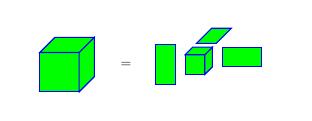
\begin{tikzpicture}[scale=0.125, every node/.style={transform shape}]
						\pgfmathsetmacro{\cubex}{4}
						\pgfmathsetmacro{\cubey}{4}
						\pgfmathsetmacro{\cubez}{4}
						\draw[blue,fill=pastelgreen] (-12,1,\cubez-2) -- ++(-\cubex,0,0) -- ++(0,-\cubey,0) -- ++(\cubex,0,0) -- cycle;
						\draw[blue,fill=pastelgreen] (-12,1,\cubez-2) -- ++(0,0,-\cubez) -- ++(0,-\cubey,0) -- ++(0,0,\cubez) -- cycle;
						\draw[blue,fill=pastelgreen] (-12,1,\cubez-2) -- ++(-\cubex,0,0) -- ++(0,0,-\cubez) -- ++(\cubex,0,0) -- cycle;
						\node[draw=none, text=black, scale=4] at (-8,-1,0) {$=$};
						
						\pgfmathsetmacro{\cubex}{2}
						\pgfmathsetmacro{\cubey}{2}
						\pgfmathsetmacro{\cubez}{2}
						\draw[blue,fill=pastelgreen] (0,0,0) -- ++(-\cubex,0,0) -- ++(0,-\cubey,0) -- ++(\cubex,0,0) -- cycle;
						\draw[blue,fill=pastelgreen] (0,0,0) -- ++(0,0,-\cubez) -- ++(0,-\cubey,0) -- ++(0,0,\cubez) -- cycle;
						\draw[blue,fill=pastelgreen] (0,0,0) -- ++(-\cubex,0,0) -- ++(0,0,-\cubez) -- ++(\cubex,0,0) -- cycle;
						
						\draw[blue,fill=pastelgreen] (-\cubex-1,1,0) -- ++(-\cubex,0,0) -- ++(0,-\cubey-2,0) -- ++(\cubex,0,0) -- cycle;
						\draw[blue,fill=pastelgreen] (\cubex+2+1,0,-\cubey) -- ++(-\cubex-2,0,0) -- ++(0,-\cubey,0) -- ++(\cubex+2,0,0) -- cycle;
						
						\draw[blue,fill=pastelgreen] (0,0,-\cubez-1) -- ++(-\cubex,0,0) -- ++(0,0,-\cubez-2) -- ++(\cubex,0,0) -- cycle;
						
						\path (-18,0) -- (8,0);
						\end{tikzpicture}
					\end{center}
				\end{block}
			\end{column}
			\begin{column}{0.305\linewidth}
				\begin{block}{\scriptsize Tensor-train decomposition}
					\begin{center}
						\begin{tikzpicture}[scale=0.125, every node/.style={transform shape}]
						
						\node (t0) at (0,-2.75) [scale=6] {$\mathcal{X}$};
						\node [scale=4]at (2.5, -2.75) {$=$};
						\path (5,-6) -- (0,0);
						\end{tikzpicture}\hspace*{-0.15cm}
						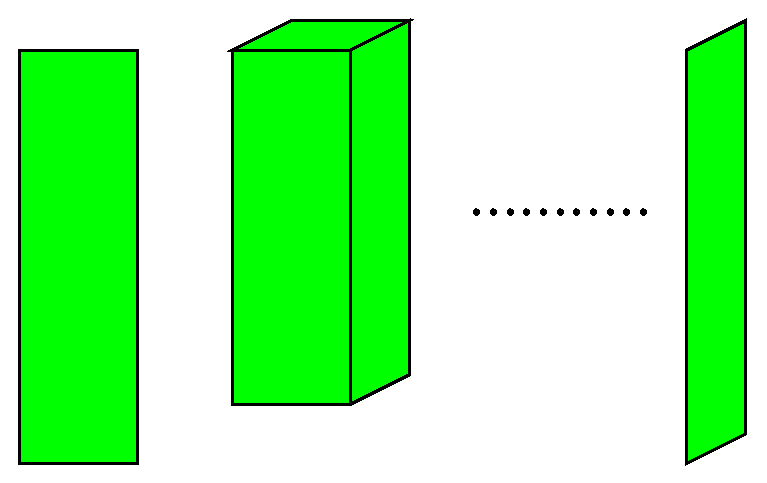
\includegraphics[scale=0.13]{./ttentry-simple.eps}
					\end{center}
					
				\end{block}
			\end{column}
		\end{columns}
	\end{center}
	
\end{itemize}

\end{frame}
\end{document} 